\documentclass[a4paper]{IEEEtran}

% Ein paar hilfreiche Pakete
\usepackage{german}
\usepackage[utf8]{inputenc}
\usepackage{graphicx} 
\usepackage{amsmath} 
\usepackage{amssymb}  
\usepackage{mathtools}
\mathtoolsset{showonlyrefs}
\usepackage{subfigure}
\usepackage{flushend}
\usepackage{url}

% Ein paar am ISAS übliche Formelzeichen
\def\rv#1{{\mathbf #1}} %Random Variable
\def\vec#1{\underline{#1}} %Vector
\def\rvv#1{{\vec{\rv{#1}}}} %Random Vector
\def\mat#1{{\mathbf #1}} %Matrix
\def\Var{\mathrm{Var}} %Variance
\def\E{\mathrm{E}} %Expectation
\def\Cov{\mathrm{Cov}} %Covariance
\def\IN{\mathrm{I\hspace{-2pt}N}} %Natural Numbers
\def\IR{\mathrm{I\hspace{-2pt}R}} %Real Numbers 

% correct bad hyphenation here
\hyphenation{op-tical net-works semi-conduc-tor}


\begin{document}
\title{Markov-Entscheidungsprozesse für die Roboterpfadplanung}

\author{Matthias~Holoch,~\IEEEmembership{E-Mail: matthias.holoch@student.kit.edu}}% <-this % stops a space




% The paper headers
\markboth{Proseminar WS 12/13: Anthropomatik: Von der Theorie zur Anwendung}%
{Proseminar WS 12/13: Anthropomatik: Von der Theorie zur Anwendung}



% make the title area
\maketitle


\begin{abstract}
Eine Aufbereitung des Markov-Entscheidungsprozess am Beispiel von autonomen Robotern. 
\end{abstract}


\section{Einleitung}
Diese Ausarbeitung beschäftigt sich mit dem Markov-Entscheidungsprozess (englisch: Markov decision process, kurz MDP), ein mathematisches Modell zur Modellierung von Entscheidungsproblemen. Es wurde nach dem russischen Mathematiker Andrey Markov benannt. Der MDP wird verwendet um Situationen, bei denen Aktionen nicht deterministische Folgen haben können zu modellieren und aus dem Modell eine Strategie, also eine Aktion für jeden Zustand, zu errechnen.

Die Erklärungen zu dem MDP werden unterstützt und motiviert durch Beispiele aus dem Bereich der autonomen Robotern. Die angeführten Beispiele basieren auf Beispielen aus \cite{thrun2005probabilistic}. Damit soll in keinster Weise impliziert werden, dass der MDP lediglich in diesem Bereich für von Interesse ist.

\begin{figure}[ht]
	\centering
	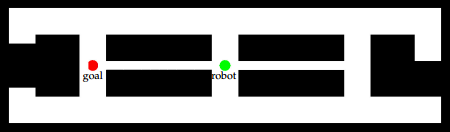
\includegraphics[scale=0.72]{images/autnmRobot_basicSituation.png}
	\caption{Eine beispielhafte Umgebung mit Roboter und Ziel. Der Roboter befindet sich mittig mit der Aufgabe sich zu dem Zielpunkt im linken Bereich der Umgebung zu bewegen. (Aus \cite{thrun2005probabilistic})}
	\label{fig:autnmRob_bSit}
\end{figure}

Wie in Abbildung \ref{fig:autnmRob_bSit} dargestellt betrachten wir im Folgenden einen autonomen Roboter der sich im Zentrum einer nahezu symmetrischen Umgebung befindet. Im linken Bereich der Umgebung befindet sich ein Ziel. Die Aufgabe des Roboters ist es, das Ziel möglichst schnell zu erreichen. Allerdings existieren mehrere Pfade die den Roboter das Ziel bringen. Einen kurzen Pfad, der durch den engen Korridor führt und zwei längere und breitere Pfade, die außen herum führen.

In einem klassischen Planungsbeispiel für Roboter existiert keine Unsicherheit. Der Roboter würde seine Position und die des Zielpunktes exakt kennen. Außerdem hätten ausgeführte Aktionen exakt vorhersehbare Effekte und solche Effekte können eingeplant werden. In so einer Situation würde vor Aktionsausführung die Vorberechnung einer Strategie, die lediglich eine einzelne Abfolge von Aktionen ist, ausreichen. Unter diesen Voraussetzungen wäre der Einbezug von Sensordaten während der Aktionsausführung unnötig, da der Roboter absolut fehlerfrei funktioniert.

\begin{figure}[ht]
	\centering
	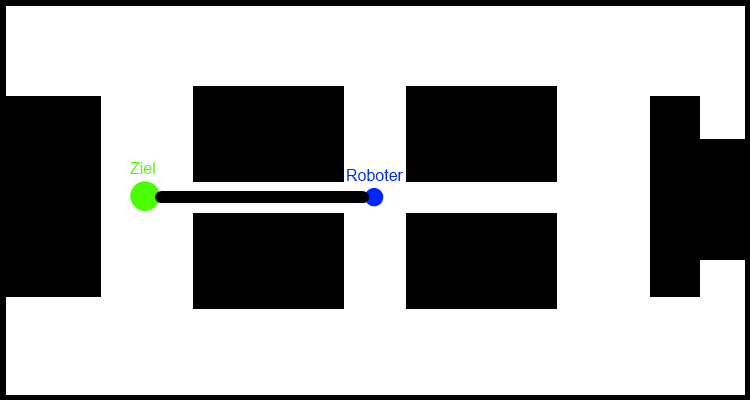
\includegraphics[scale=0.72]{images/autnmRobot_directPath.png}
	\caption{Ohne die Anwesenheit von Fehlern in der Bewegung des Roboters ist der kürzere, enge Pfad dem längeren, breiten Pfad klar überlegen. (Aus \cite{thrun2005probabilistic})}
	\label{fig:autnmRob_dirPath}
\end{figure}

Abbildung \ref{fig:autnmRob_dirPath} zeigt eine solche vorberechnete Strategie. Da bisher angenommen wurde, dass der Roboter absolut fehlerfrei funktioniert ist der kürzere, enge Pfad jedem der längeren, breiten Pfade vorzuziehen.

In der Praxis funktionieren solche Strategien meist aus mehreren Gründen nicht richtig: Ein Roboter, der blind einem engen Korridor folgt läuft Gefahr mit den Wänden zu kollidieren. Außerdem ist es sehr wahrscheinlich, dass der Roboter auf Grund des während der Aktionsausführung akkumulierten Fehlers das Ziel verfehlt.

Daher werden in der Praxis häufig Planungsalgorithmen dieser Art mit einem sensorbasierten Kontrollmodul kombiniert. Dieses Kontrollmodul verwendet die Sensordaten des Roboters um Fehler, die bei der Aktionsausführung auftreten, zu erkennen und den Roboter immer wieder auf den geplanten Kurs zurück zu führen. Insbesondere bei einem Fall wie dem engen Korridor in unserem Beispiel muss so eine Korrektur besonders häufig stattfinden, um eine Kollision mit der Wand des Korridors zu vermeiden. Dadurch ergibt sich eine signifikante Verringerung der Fortbewegungsgeschwindigkeit des Roboters, die von dem klassischen Planungsalgorithmus nicht berücksichtigt wird. 

\begin{figure}[ht]
	\centering
	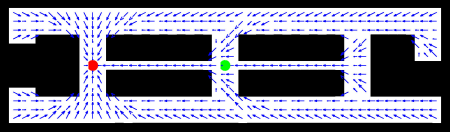
\includegraphics[scale=0.72]{images/autnmRobot_detActionMDP.png}
	\caption{Darstellung einer Strategie bei \emph{nicht} probabilistischen Effekten bei der Aktionsausführung. Hier ist der kurze Pfad klar überlegen. (Aus \cite{thrun2005probabilistic})}
	\label{autnmRobot_detA}
\end{figure}
\begin{figure}
	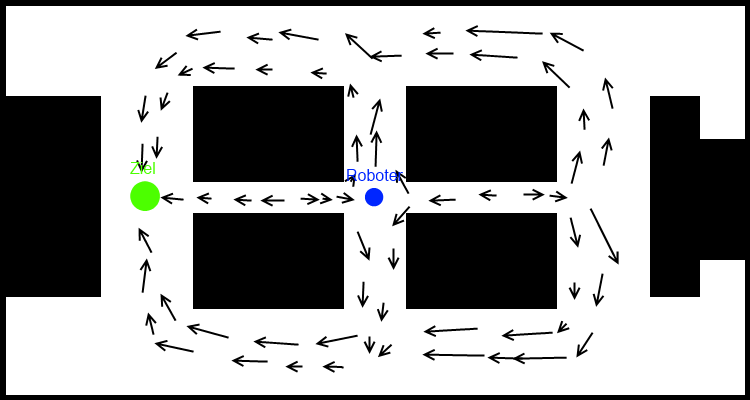
\includegraphics[scale=0.72]{images/autnmRobot_ndetActionMDP.png}
	\caption{Darstellung einer Strategie bei probabilistischen Effekten bei der Aktionsausführung. Hier wird der längere Pfad bevorzugt. (Aus \cite{thrun2005probabilistic})}
	\label{autnmRobot_ndetA}
\end{figure}

Als Konsequenz muss eine robustere Strategien nicht lediglich eine einzelne Aktionsabfolge vorberechnen, sondern mehrere Aktionen für eine Vielfalt an Situationen, in die der Roboter auf Grund seiner unvorhersehbaren, fehlerbehafteten Aktionsausführung geraten könnte.

Um eine solche Strategie vorberechnen zu können benötigen wir ein Modell, welches stochastische Effekte in der Aktionsausführung erlaubt. Ein solches Modell ist der MDP. Eine aus einem MDP berechnete Strategie gibt für jeden Zustand der Umgebung, hier der Ort, an dem sich der Roboter befindet, eine bestmögliche Aktion an. In diesem Beispiel ist eine solche Aktion eine Bewegung in eine bestimmte Richtung. Egal ob bei der Bewegung Fehler auftreten oder nicht, der Roboter kann danach mit seinen Sensoren seinen Ort erneut feststellen und findet in der vorberechneten Strategie eine nächste optimale Aktion.

Abbildung \ref{autnmRobot_detA} zeigt eine solche Strategie für einen Roboter mit fehlerfreier Aktionsausführung. Hier wählt die Strategie bevorzugt den Weg durch den engen, kurzen Korridor. In Abbildung \ref{autnmRobot_ndetA} ist eine Strategie für einen Roboter mit fehlerbehafteter Aktionsausführung dargestellt. Hier wird hingegen einer der längeren, breiten Pfade bevorzugt.

Allerdings setzt der MDP voraus, dass der Agent, in unserem Beispiel der Roboter, den Zustand der Umgebung zu jedem Zeitpunkt exakt erkennen kann. Wir müssten also annehmen, dass die Sensoren des Roboters perfekt funktionieren.

In der Praxis ist natürlich auch diese Annahme nicht haltbar. Jedes Sensormodul hat mehr oder weniger stark ausgeprägtes Fehlerrauschen. Bei den meisten Anwendungen, wie auch bei unserem Beispiel, kommt sogar noch ein weiteres Problem hinzu: Falls der Roboter nicht über äußerst ausgeklügelte Positionsbestimmungssensoren verfügt, dann ist es ihm auf Grund der Symmetrie der Beispielumgebung nicht möglich festzustellen, wie er orientiert ist und damit in welcher Richtung das Ziel liegt.

Ein solches Modell, der teilweise beobachtbare Markov-Entscheidungsprozess (englisch: partially observable Markov decision process, kurz: POMDP), wird im vierten Kapitel dieser Ausarbeitung kurz angerissen.

\section{MDP}
\begin{figure}[ht]
	\centering
	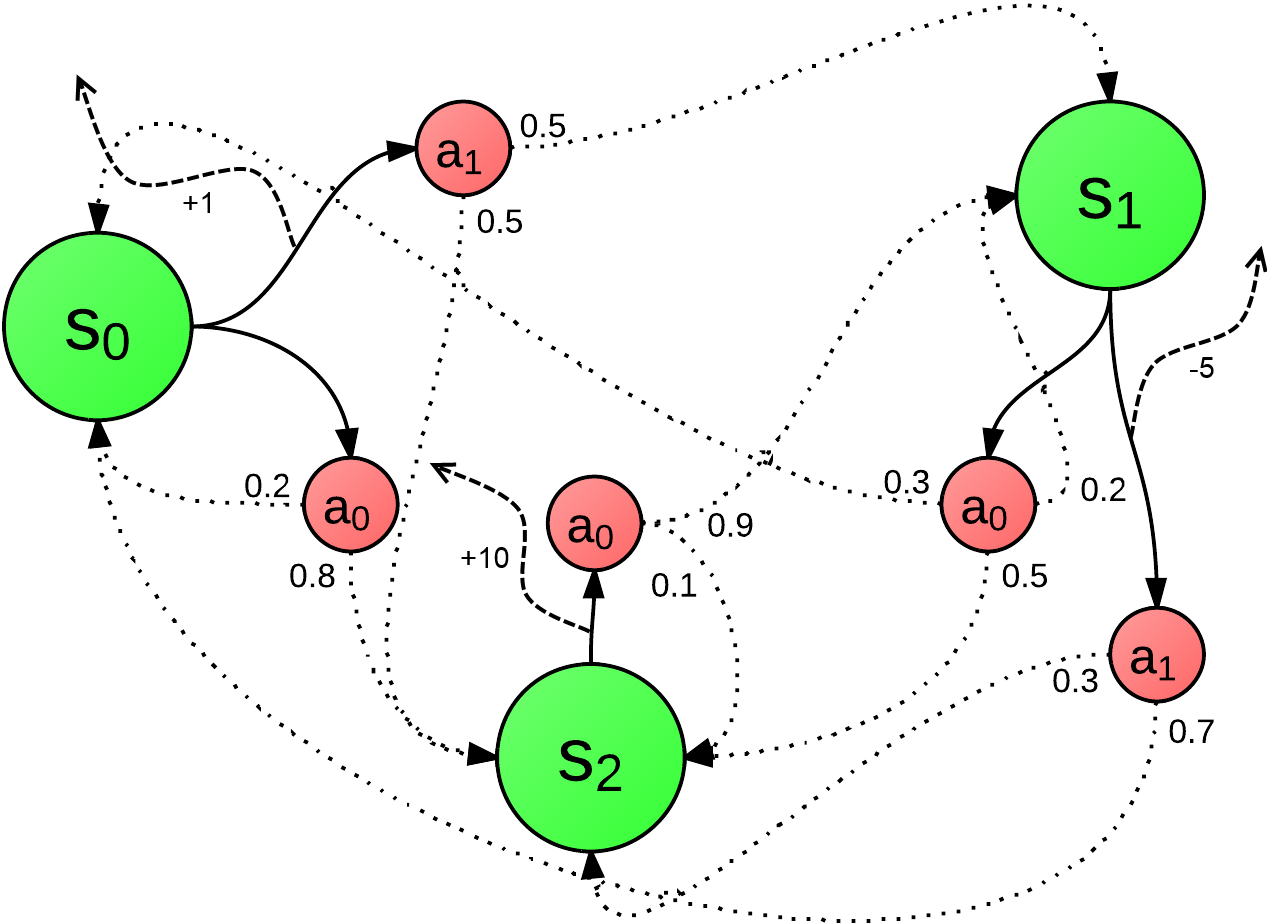
\includegraphics[scale=0.42]{images/MDP_example.png}
	\caption{Beispiel eines simplen MDP mit drei Zuständen $s_1, s_2, s_3$ und zwei Aktionen $a_0$ und $a_1$ dargestellt als Graph.}
	\label{fig:MDP_example} %TODO Dieses Bild ist durch die Änderung der Definition nicht mehr passend. Am besten selbst ein Bild machen.
\end{figure}
Nach \cite{cassandra1995acting} ist ein MDP definiert als ein 4-Tupel
\begin{equation}
	(S, A, T, R) \ .
\end{equation}
Es gibt also folgende vier grundlegende Komponenten:
\begin{enumerate}
	\item Die endliche Zustandsmenge $S$ beinhaltet alle möglichen Zustände, in denen sich die Umgebung befinden kann. Der Agent kann jederzeit exakt feststellen, in welchem Zustand sich die Umgebung befindet.
	\item Die endliche Menge der Aktionen $A$. In jedem Zustand kann der Agent aus einer Menge $A_s \subseteq A$ von ausführbaren Aktionen wählen.
	\item $T$ ist das Zustandsübergangsmodell der Umgebung. Es ist eine Funktion, welche Elemente aus $S \times A$ auf eine diskrete Wahrscheinlichkeitsverteilung über $S$ abbildet. Der Übergang
	\begin{equation}
		p(s, a, s')
	\end{equation}
	drückt die Wahrscheinlichkeit aus, dass sich die Umgebung nach Wählen der Aktion $a$ in Zustand $s$ im Zustand $s'$ befindet.
	\item Die Gütefunktion
	\begin{equation}
		r: S \times A \rightarrow \IR
		\label{eq:payoff}
	\end{equation}
	drückt die sofortige Belohnung bzw. die sofortigen Kosten (englisch: payoff) für den Agenten in Abhängigkeit von der gewählten Aktion in einem Zustand aus. Kosten werden als negative Zahlen und Belohnungen als positive Zahlen dargestellt.
\end{enumerate}
In Abbildung \ref{fig:MDP_example} ist ein MDP mit drei Zuständen $s_1, s_2, s_3$ und zwei Aktionen $a_0$ und $a_1$ als Graph dargestellt. Für jeden Zustand $s \in S$ gibt es eine Teilmenge $A_s \subseteq A$ von Aktionen von denen ausgehende Kante die Wahrscheinlichkeit des Übergangs in den entsprechenden Folgezustand als Kantengewicht darstellen. Die gelben Pfeile symbolisieren die Belohnung bzw. die Kosten (siehe \ref{eq:payoff}) für bestimmte Aktionen in bestimmten Zuständen.

In mancher Literatur finden sich auch leicht anders geartete Definitionen. In \cite{russell1995artificial} ist beispielsweise die Gütefunktion eine Funktion, die lediglich von dem Zustand abhängt und es gibt eine Teilmenge $S_{terminal} \subseteq S$ der Zustandsmenge die als Terminalzustände bezeichnet werden. Sobald sich der Agent in einem Terminalzustand befindet kann er keine Aktionen mehr durchführen. Dadurch kann die Modellierungen bestimmter Umgebungen vereinfacht werden, verändert das Problem nur unwesentlich.


\section{Strategien aus dem MDP}
\subsection{Motivation}
Nun haben wir ein Modell kennengelernt, mit dem wir Unsicherheit in der Aktionsausführung korrekt modellieren können. Damit der Roboter aus unserem Beispiel tatsächlich etwas mit dieser Art der Modellierung anfangen kann, müssen wir einen Weg finden aus dem Modell eine Strategie vor zu berechnen. Wie wir schon erkannt haben reicht dazu eine festgelegte Sequenz an Aktionen nicht aus. Stattdessen muss eine Strategie für jeden möglichen Zustand festlegen, was zu tun ist. Eine gängige Bezeichnung einer Strategie (englisch: policy) ist
\begin{equation}
	\pi:S \rightarrow A
	\label{eq:policy}
\end{equation}
und $\pi(s)$ ist die von der Strategie $\pi$ vorgeschlagene Aktion im Zustand $s$. Hat der Roboter eine solche Strategie ist immer klar was er als nächstes zu tun hat - unabhängig davon, was bei der Aktionsausführung tatsächlich geschieht.

\subsection{Optimale Strategie}
Ein wichtiges Konzept im Kontext von Strategien ist der Planungshorizont. (englisch: planning horizon) In manchen Fällen kann es reichen eine Strategie so zu wählen, dass die unmittelbare Belohnung maximiert wird. In den meisten Fällen zahlen sich Aktionen aber nicht sofort aus. In unserem Beispiel wäre eine Gütefunktion
\begin{equation}
	r(s,a) = \left\{ \begin{array}{rl}
		+100 &\mbox{ falls $a$ in das Ziel führt} \\
		-1 &\mbox{ sonst}
       \end{array} \right.
\end{equation}
denkbar. Hier wird deutlich erkennbar, dass die Belohnung erst nach vielen Aktionen eintritt. Daher kann eine Strategie, die lediglich die unmittelbare Belohnung maximiert hier kein optimales Ergebnis liefern: Jede Aktion, egal ob sie in Richtung des Ziels oder vom Ziel weg führt hat die Kosten -1 und wären somit für eine solche Strategie gleichwertig.
Stattdessen setzt man sich häufig zum Ziel die Summe der zukünftigen Belohnungen zu maximieren.

Die folgenden Ausführungen basieren auf \cite{russell1995artificial}. Zunächst müssen wir uns über den Wert bzw. der Nützlichkeit (englisch: utility) einer Aktionsfolge 
\begin{equation}
	U([(s_0, a_0), (s_1, a_1), ..., (s_n, a_n)])
\end{equation}
klar werden. Ist unser Planungshorizont endlich, dann gibt es einen Zeitpunkt $n \in N$ nach dem Aktionen des Agenten nichts mehr Wert sind. Demnach ist 
\begin{equation}
	\begin{split}
		U([ (s_0, a_0), (s_1, a_1), ..., (s_n, a_n)]) \\
		= U([ (s_0, a_0), (s_1, a_1), ..., (s_{n+k}, a_{n+k})]),\\
		\forall k \in \IN \ .
	\end{split}
\end{equation}
Dadurch kann es vorkommen, dass beispielsweise ein Zielpunkt mit besonders hoher Belohnung zu einem bestimmten Zeitpunkt von manchen Zuständen aus nicht mehr erreicht werden kann und daher die optimale Aktion in diesem Zustand eine andere ist, als wäre der Agent zu einem früheren Zeit in diesem Zustand gewesen. Daher kommt der Effekt, dass bei einem endlichen Planungshorizont sich die optimale Aktion in demselben Zustand über die Zeit ändern kann. Die optimale Strategie für einen endlichen Planungshorizont ist nicht stationär. (englisch: nonstationary)

Diese Problematik existiert nicht, wenn wir einen unendlichen Planungshorizont annehmen. Dann gibt es keinen Grund zu verschiedenen Zeitpunkten eine andere Aktion in demselben Zustand zu wählen.

Es gibt mehrere Möglichkeiten einer Aktionsfolge einen Wert zuzuweisen:
\begin{enumerate}
	\item \textbf{Additive Güte:} (englisch: additive rewards)
		\begin{equation}
			U([ (s_0, a_0), (s_1, a_1), ..., (s_n, a_n)]) = \sum\limits_{t=1}^n r(s_t, a_t)\ .
		\end{equation}
		Die additive Güte funktioniert nur dann gut, wenn der Planungshorizont endlich ist. Bei einem unendlichen Planungshorizont ($n \rightarrow \infty$) divergiert die Wertefunktion und zwei Aktionsfolgen können nicht mehr unterschieden werden. Als anschauliches Beispiel kann man sich zwei Arbeitsplätze vorstellen, von denen uns der eine 1 Geldeinheit pro Stunde einbringt und der andere 10 Geldeinheiten pro Stunde. Bei unendlichem Planungshorizont bringen beide Jobs unendlich viel Geldeinheiten ein und sind dadurch für die Strategie gleichwertig.
	\item \textbf{Reduzierte Güte:} (englisch: discounted rewards)
		\begin{equation}
			\begin{split}
				U([ (s_0, a_0), (s_1, a_1), ..., (s_n, a_n)]) = \sum\limits_{t=1}^n \gamma^t r(s_t, a_t),\\
				\text{mit }\gamma \in [0,1]\ .
			\end{split}
		\end{equation}
		Der Reduzierungsfaktor $\gamma$ (englisch: discount factor) drückt aus, wie wichtig die zeitliche Nähe der Belohnung ist. Für $\gamma=1$ lässt sich mit der reduzierten Güte auch das additive Modell darstellen. Die additive Güte ist also ein Spezialfall der reduzierten Güte. Nach \cite{thrun2005probabilistic} gilt für $\gamma < 1$ und bei beschränkter Güte 
		\begin{equation}
			\exists r_{max} \in \IR\ \forall s \in S\ \forall a \in A: |r(s,a)| < r_{max} \ ,
		\end{equation}
		dass die Wertefunktion auch bei unendlichem Planungshorizont konvergiert. Die Güte lässt sich dann abschätzen mit  
		\begin{equation}
			\sum\limits_{t=1}^n \gamma^t r(s_t, a_t) \leq \sum\limits_{t=1}^n \gamma^t r_{max} = \frac{r_{max}}{1-\gamma}  \ .
		\end{equation}
	\item
		Eine weitere Möglichkeit bei unendlichem Planungshorizont wäre die durchschnittliche Güte pro Zeitschritt zu betrachten, sprengt aber den Rahmen dieser Ausarbeitung.
\end{enumerate}
Zusammenfassend ist die Verwendung von reduzierter Güte mit den wenigsten Problemen verbunden, um mit ihr den Wert einer Aktionsfolge zu bewerten.

Der letzte Schritt ist nun die beste Strategie $\pi$ zu wählen, wobei wir im Kopf behalten müssen, dass eine Strategie nicht nur eine Aktionsfolge bedeutet, sondern eine ganze Reihe von möglichen Aktionsfolgen. Daher ist der Wert einer Strategie die erwartete Summe der reduzierten Güte aller Aktionsfolgen, die $\pi$ generieren könnte. Eine optimale Strategie ist
\begin{equation}
	\pi^* = \underset{\pi}{argmax}\ \E \left[ \sum\limits_{t=1}^{\infty} \gamma^t r(s_t, a_t) \ \vert\ \pi \right]\ .
\end{equation}

\subsection{Value iteration} %TODO german title?
Nun da wir wissen wie eine optimale Strategie aussieht müssen wir nur noch eine Möglichkeit finden eine solche mit einem konkreten Algorithmus zu erzeugen. In Anlehnung an \cite{thrun2005probabilistic} folgt nun ein value iteration Algorithmus, der genau das bewerkstelligt. %TODO "value iteration" - german?

Dazu betrachten wir zunächst einen beschränkten Planungshorizont. Eine optimale Strategie 
\begin{equation}
	\pi_1^*: s \rightarrow a
\end{equation}
für einen Planungshorizont $n=1$ ist sehr einfach zu finden, in dem man für jeden Zustand jene Aktion wählt, welche die höchste Güte liefert
\begin{equation}
	\pi_1^*(s)= \underset{a}{argmax}\ r(s, a)
\end{equation}
Außerdem definieren wir zu diesem Planungshorizont eine Wertefunktion, die jedem Zustand einen erwarteten Wert zuweist. Diese Wertefunktion
\begin{equation}
	V_1(s) = \gamma\ \underset{a}{max}\ r(s, a)
\end{equation}
ist der reduzierte Wert der höchsten Belohnung, die eine der möglichen Aktionen liefert.

Für den Planungshorizont $n=2$ können wir nun auf die für den Planungshorizont $n=1$ schon definierten Funktionen aufbauen. Die optimale Strategie für $n=2$ wählt für jeden Zustand $s$ jene Aktion $a$, welche die Summe aus der sofortigen Belohnung $r(s,a)$ und der erwarteten Belohnung aus der Wertefunktion $V_1(s)$ maximiert
\begin{equation}
	\pi_2^*(s) = \underset{a}{argmax} \left[ r(s,a) + \sum_{s' \in S} V_1(s')\ p(s, a, s') \right]\ .
\end{equation}
Die entsprechende Wertefunktion lautet dann
\begin{equation}
	V_2(s) = \gamma\ \underset{a}{max} \left[ r(s,a) + \sum_{s' \in S} V_1(s')\ p(s, a, s') \right]\ .
\end{equation}

Um nun eine optimale Strategie bzw. eine Wertefunktion für einen beliebigen Planungshorizont $n,\text{ mit }n > 1$ zu berechnen lässt sich rekursiv auf schon berechnete Wertefunktionen aufbauen.
\begin{equation}
	\pi_n^*(s) = \underset{a}{argmax} \left[ r(s,a) + \sum_{s' \in S} V_{n-1}(s')\ p(s, a, s') \right]\
\end{equation}
\begin{equation}
	V_n(s) = \gamma\ \underset{a}{max} \left[ r(s,a) + \sum_{s' \in S} V_{n-1}(s')\ p(s, a, s') \right]\
\end{equation}

Für einen unendlichen Planungshorizont neigt die Wertefunktion %TODO Nach Buch..?
\begin{equation}
	V_\infty(s) = \gamma\ \underset{a}{max} \left[ r(s,a) + \sum_{s' \in S} V_{\infty}(s')\ p(s, a, s') \right]\
\end{equation}
dazu irgendwann ein Gleichgewicht zu erreichen. Diese Invarianz ist als \emph{Optimalitätsprinzip von Bellman} bekannt.

Diese Überlegungen führen uns zu einem konkreten Algorithmus, der aus einem MDP mit endlicher Zustandsmenge bei unendlichem Planungshorizont eine näherungsweise optimale Strategie berechnet. Unsere angenäherte Wertefunktion $\hat{V}$ initialisieren wir der kleinstmöglichen Güte $r_{min}$ %TODO Unsinn, das mit r_min zu machen? Warum nicht mit 0?
\begin{equation}
	\forall s \in S:\hat{V}(s) \leftarrow r_{min}\ .
\end{equation}
Daraufhin wird die Wertefunktion rekursiv mit
\begin{equation}
	\hat{V}(s) \leftarrow \gamma\ \underset{a}{max} \left[ r(s,a) + \sum_{s' \in S} \hat{V}(s')\ p(s, a, s') \right]\
\end{equation}
aktualisiert, bis die Wertefunktion konvergiert. Im Allgemeinen geschieht das nur für $\gamma < 1$, in einigen Spezialfällen auch für $\gamma = 1$.

Zu jedem Zeitpunkt induziert die Wertefunktion $\hat{V}$ die Strategie
\begin{equation}
	\pi(s) = \underset{a}{argmax} \left[ r(s,a) + \sum_{s' \in S} \hat{V}(s')\ p(s, a, s') \right]\
\end{equation}
Abbildung \ref{autnmRobot_policy} zeigt eine auf diese Weise berechnete Wertefunktion für unser Beispiel. Diese Wertefunktion induziert die Strategie, die in Abbildung \ref{autnmRobot_detA} dargestellt ist.

\begin{figure}[ht]
	\centering
	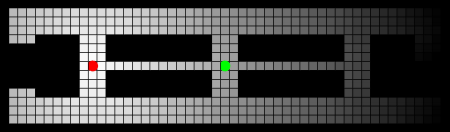
\includegraphics[scale=0.72]{images/autnmRobot_MDPValueFunction.png}
	\caption{Ein Beispiel einer Wertefunktion bei unendlichem Planungshorizont. Diese Wertefunktion induziert die Strategie in Abbildung \ref{autnmRobot_detA} (Aus \cite{thrun2005probabilistic})}
	\label{autnmRobot_policy}
\end{figure}

\section{Ausblick}
\subsection{POMDP}
\begin{figure}[ht]
	\centering
	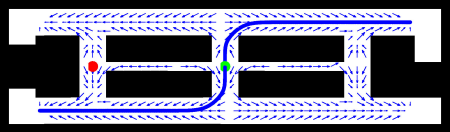
\includegraphics[scale=0.72]{images/autnmRobot_POMDPPathA.png}
	\caption{Die Strategie zu einem Zeitpunkt, an dem die Orientierung des Roboters noch nicht feststeht. Um zu vermeiden, auf Grund der Symmetrie der Umgebung in die falsche Richtung zu fahren ist es sinnvoll an den linken bzw. den rechten Rand der Umgebung zu fahren, die sich deutlich unterscheiden. (Aus \cite{thrun2005probabilistic})}
	\label{autnmRobot_POMDPPathA}
\end{figure}

\begin{figure}[ht]
	\centering
	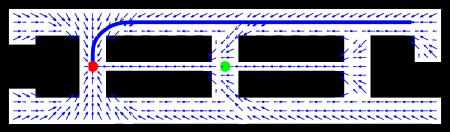
\includegraphics[scale=0.72]{images/autnmRobot_POMDPPathB.png}
	\caption{Die Strategie zu dem Zeitpunkt, an dem durch den Markanten Punkt am rechten Rand der Roboter den Ort des Zieles mit sehr hoher Wahrscheinlichkeit kennt. (Aus \cite{thrun2005probabilistic})}
	\label{autnmRobot_POMDPPathB}
\end{figure}

\begin{figure}[ht]
	\centering
	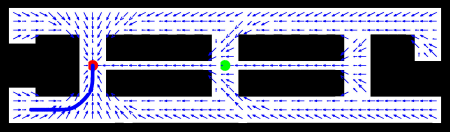
\includegraphics[scale=0.72]{images/autnmRobot_POMDPPathC.png}
	\caption{Die Strategie zu dem Zeitpunkt, an dem durch den Markanten Punkt am linken Rand der Roboter den Ort des Zieles mit sehr hoher Wahrscheinlichkeit kennt. (Aus \cite{thrun2005probabilistic})}
	\label{autnmRobot_POMDPPathC}
\end{figure}

Bisher nahmen wir an, dass die Sensoren des Roboters jederzeit den exakten Zustand der Umgebung wahrnehmen können. In der Praxis liefern Sensoren allerdings lediglich ein verrauschtes Abbild der Umgebung. Daher kann der Zustand nur bis zu einem gewissen Grade geschätzt werden.

Um diese Problematik zu veranschaulichen betrachten wir nun wieder unsere Beispielanwendung. Das einzige Unterscheidungsmerkmal findet sich am linken bzw. rechten Ende der Umgebung. Direkt in Richtung eines möglichen Zielortes zu fahren würde eine 50\% Chance mit sich bringen das Ziel zu verpassen und stattdessen zu dem entsprechenden Ort auf der anderen Seite zu fahren. Optimalerweise muss der Roboter nun also zuerst in eine der Ecken fahren um sicher feststellen zu können, wo sich das genau Ziel befindet. (Das Ziel selbst ist für die Sensoren des Roboters nicht wahrnehmbar)

Stichpunktartig: %TODO

Schlüsselaspekt bei probabilistic robotics: Der Roboter führt information gather tasks aus (hier das fahren in eine der Ecken)

Wir benötigen also ein Modell, in dem der Zustand der Umgebung nicht mehr vollständig beobachtbar sein muss. (Wahrscheinlichkeitsverteilung über die Zustände..?)

Strategien generieren, die auf dem belief state oder information space arbeiten. Eine solche Strategie für unser einfaches Beispiel ist in Abbildungen \ref{autnmRobot_POMDPPathA}, \ref{autnmRobot_POMDPPathB}, \ref{autnmRobot_POMDPPathC} zu sehen.

Unterschied zu MDP: Es ist nie klar, in welchem Zustand man sich befindet. Stattdessen gibt es eine Funktion, die eine Wahrscheinlichkeitsverteilung über die Zustände beschreibt.

\subsection{Strategien aus POMDP}
Idee ein POMDP als Coninuous Space MDP zu sehen. --> Value Iteration artig lösen.

Eine kleine Liste von weiteren (teilweise approximativen) Algorithmen. Dafür versuche ich am besten auch noch ein Papier zu finden, auf das ich dazu referenzieren kann.

\section{Weitere Anwendungsgebiete}
Natürlich ist der MDP bzw. der POMDP nicht nur für die Aktionsplanung von autonomen Robotern interessant. In \cite{cassandra1998survey} werden eine Reihe von verschiedenen möglichen Anwendungsgebieten diskutiert. Die dort beleuchteten Anwendungsgebiete sind
\begin{itemize}
	\item Industrielle Anwendungsgebiete
	\begin{itemize}
		\item Wartung von Maschinen
		\item Struktur-Inspektion
		\item Aufzugsteuerungsstrategien
	\end{itemize}
	\item Wissenschaftliche Anwendungsgebiete
	\begin{itemize}
		\item Autonome Roboter
		\item Verhaltensökologie
		\item Maschinelles Sehen
	\end{itemize}
	\item Gewerbliche Anwendungsgebiete
	\begin{itemize}
		\item Fehlerbehebung in Netzwerken
		\item Anfragen auf verteilte Datenbanken
		\item Marketing
		\item Entwurf von Fragebögen
		\item Geschäftspolitik
	\end{itemize}
	\item Militärische Anwendungsgebiete
	\begin{itemize}
		\item Moving Target Search %TODO deutsche Übersetzung?
		\item Search and Rescue
		\item Target Identification
		\item Weapon Allocation
	\end{itemize}
	\item Gesellschaftliche Anwendungsgebiete
	\begin{itemize}
		\item Bildung
		\item Medizinische Diagnose
		\item Gesundheitspolitik
	\end{itemize}
\end{itemize}

%%%%%%%%%%%%%%%%%%%%%%%%%%%%%%%%%%%%%%%%%%%%%%%%%%%%%%%%%%%%%%%%%%%%%%%%%
% Literaturverzeichnis (in literatur.bib, z.B. mit Jabref editieren) 
\bibliographystyle{plain}
\bibliography{literatur}
\end{document}